\documentclass[]{IEEEtran}

\title{Modellazione e Sintesi di un Moltiplicatore Floating-point Single Precision}
\author{Elena Ramon}

\usepackage{graphicx}
\usepackage[italian]{babel}

\begin{document}
\maketitle

\begin{abstract}
In questo documento viene presentato un sistema per il calcolo del prodotto in virgola mobile a singola precisione.
\end{abstract}

\section{Introduzione}

Il sistema che viene descritto di seguito si occupa di eseguire il calcolo di due moltiplicazioni in virgola mobile. Una rappresentazione astratta del sistema è quella in figura \ref{fig:abstract}, dove:
\begin{itemize}
    \item Top level: si occupa di sincronizzare i due moltiplicatori. Esso funge da interfaccia tra l’ambiente esterno e i sottocomponenti. Per simulare l’ambiente esterno è stato progettato un testbench. 
    
    \item Moltiplicatori: si occupano dell'esecuzione del prodotto in virgola mobile. 
\end{itemize}

Per giungere alla soluzione finale inizialmente è stato scritto lo pseudocodice dell’algoritmo per la moltiplicazione in virgola mobile, in tal modo è stato possibile identificare le porte ed i segnali dei sottocomponenti (i moltiplicatori) e del toplevel. Questo ha permesso inoltre di redigere più facilmente le EFSM (extended finite state machine) del moltiplicatore e del top level, le quali sono state sviluppate nel seguente ordine moltiplicatore e top level. Il sistema è stato presentato in due versioni, una che utilizza VHDL e verilog (due linguaggi di descrizione dell’hardware) e una che utilizza SystemC (un insieme di librerie di C++). Per la prima versione si è scelto di sviluppare il top level e il testbench in VHDL.

\section{Background}
Il sistema è stato sviluppato in due versioni, una in VHDL/verilog e una in SystemC, entrambe utilizzando RTL (register transfer level) come livello di astrazione. Dunque top level e moltiplicatori sono stati suddivisi in due processi, uno che si occupa di controllare il flusso di esecuzione (fsm) e uno che si occupa di eseguire le operazioni logico/aritmetiche (datapath).

VHDL e verilog sono due linguaggi di descrizione dell’hardware (HDL). Si presentano come dei normali linguaggi di programmazione, con la differenza che permettono di simulare processi concorrenti. SystemC è anch’esso un linguaggio di descrizione dell’hardware (HDL). Si presenta come un insieme di librerie di C++, che aggiungono la possibilità di simulare processi concorrenti.

È stata poi implementata una versione che permette di effettuare la HLS (high level synthesis). è stata scritta una funzione in C++ che effettua la moltiplicazione di due float, la quale è stata poi sintetizzata usando VIVADO HLS [todo]. Questo tipo di sintetizzazione interpreta una descrizione algoritmica creando l’implementazione in hardware digitale. 

\section{Metodologia applicata}

Il sistema è suddiviso in due moduli, quello che si occupa della moltiplicazione in virgola mobile (rappresentato nel sistema come due sottocomponenti che eseguono due moltiplicazioni differenti) e il top level che si occupa di sincronizzare i due sottocomponenti.

\subsection{Moltiplicatore}
\ref{fig:efsmmul}Durante la fase di ricezione degli operandi il modulo li divide nelle diverse componenti (segno, esponente e mantissa) che vengono memorizzate in 3 diversi segnali per ogni operando. Prima di procedere con la moltiplicazione il modulo verifica che gli operandi che ha ricevuto in ingresso siano ben formati, cioè che non si tratti di NaN (esponente con tutti i bit a 1 e mantissa diversa da 0) o di denormalizzati (esponente con tutti i bit a 0 e mantissa diversa da 0), e che non si tratti di moltiplicazioni “semplici”. Con “semplici” ci si riferisce ai casi 0 * 0 = 0, Inf * Inf = Inf, 0 * Inf = NaN, 0 * num = 0, Inf * num = Inf.  Nel caso di operandi mal formati il risultato si presenta come 32 bit a 0 e un valore diverso da 0 sul segnale dell’eccezione. Le eccezioni rappresentate sono le seguenti:
\begin{itemize}
	\item NaN : 001
	\item Denormalize : 010	
	\item NaN e Denormalize : 011 (si presenta quando un operando è NaN e uno è denormalizzato. Le due eccezioni separatamente esistono, ma visto che si può verificare il caso in cui si presentano entrambe contemporaneamente e che il controllo sugli operandi viene fatto simultaneamente ed è l’unico caso che si verifica, è stata scelta una codifica a parte per rappresentarlo)
	\item Overflow : 100
	\item Underflow : 101
\end{itemize}

Nel caso invece in cui sia tutto ok viene calcolato l’esponente del risultato e la moltiplicazione tra le mantisse. Dopo aver calcolato l’esponente viene controllato che non si siano verificati overflow o underflow. Una volta effettuato il prodotto si verifica che la mantissa sia ancora normalizzata, altrimenti si procede con la normalizzazione (incremento dell’esponente e shift della mantissa). Viene poi eseguito l’arrotondamento utilizzando l’algoritmo “round to nearest ties to even”, secondo il quale se la parte dopo l’ultima cifra significativa è a “metà via” viene eseguito l’arrotondamento verso la cifra pari più vicina.  Questo procedimento può essere eseguito più volte, visto che ogni modifica fatta può richiederne altre. Una volta ultimati i controlli il modulo immette il risultato sulle porte. 
\ref{fig:fsmdmul}Le porte di ingresso e di uscita sono le seguenti:
\begin{itemize}
    \item clk : in bit
    \item rst : in bit
    \item ready : in bit
    \item op : in unsigned 32 bit
    \item done : out bit
    \item eccezione\_out : out unsigned 3 bit
    \item result : out unsigned 32 bit
\end{itemize}
Mentre i segnali utilizzati sono:
\begin{itemize}
	\item current\_state e next\_state : rappresentano lo stato attuale e il successivo della EFSM
	\item mantissa\_op1 e mantissa\_op2 : unsigned 24 bit, usati per memorizzare la mantissa degli operatori con il MSB a 1 (il bit implicito seguito dalla virgola e poi dai 23 bit della mantissa, necessario per la moltiplicazione)
	\item esponente\_op1 ed esponente\_op2 : unsigned 8, usati per memorizzare l’esponente degli operatori
	\item segno\_op1 e segno\_op2 : bit, usati per memorizzare il segno degli operatori
	\item t7 ed esponente: unsigned 9 bit, vengono usati per il calcolo del nuovo esponente, t7 rappresenta il valore temporaneo che contiene la somma dei due esponenti in ingresso; esponente invece rappresenta il t7 - 127. Sono entrambi a 9 bit perché la somma e la sottrazione possono produrre overflow
	\item mantissa: unsigned 25 bit, rappresenta il possibile risultato finale della moltiplicazione. Vengono utilizzati 25 bit perché 24 rappresentano la mantissa con il bit implicito, mentre il 25-esimo serve per verificare l’eventuale overflow dovuto alla somma nella fase di arrotondamento della mantissa
	\item moltiplicando e temp\_mantissa : unsigned 48 bit, moltiplicando viene utilizzato durante la moltiplicazione delle mantissa, inizialmente contiene mantissa\_op1, ha una lunghezza di 48 bit in quanto durante la moltiplicazione viene eseguito uno shift a sinistra 24 volte (pari al numero di bit delle mantisse). temp\_mantissa contiene i risultati intermedi (e finale) della moltiplicazione e viene usato nella fase di normalizzazione per effettuare l’arrotondamento.
	\item counter : integer, viene usato durante la moltiplicazione per effettuare un numero di cicli pari a 24 (il numero di bit delle mantisse)
	\item eccezione: unsigned 3 bit, viene usata per memorizzare nei passi intermedi il codice dell’eccezione che si è verificata
	\item t1, t2, t3, t4, t5, t6 : bool, vengono usati per effettuare i controlli iniziali sugli esponenti e le mantisse e per i controlli sull’arrotondamento della mantissa risultato
\end{itemize}
Come detto in precedenza il moltiplicatore è suddiviso in due processi che rappresentano FSM e datapath. Il primo è un processo con sensitivity list che contiene tutti i segnali letti che sono ready, t1, t2, t3, t4, t5,t6, counter, temp\_mantissa, esponente, mantissa, current\_state i quali vengono utilizzati nei diversi stati per decidere lo stato prossimo. Il datapath è un processo con sensitivity list che contiene il clock e il reset.

\subsection{Top level}
\ref{fig:efsmtl}Il top level si occupa di sincronizzare i due moltiplicatori. Gli operandi passano dalle sue porte direttamente ai sottocomponenti, è stato deciso che i 2 operandi vadano uno ad un sottocomponente e uno all'altro. Quindi attende che i moltiplicatori terminino la loro esecuzione. Per tale motivo usa i segnali done\_VHDL e done\_verilog. Nel caso in cui entrambi valgano 1 contemporaneamente e quindi entrambi i sottocomponenti abbiano terminato la loro esecuzione esso invia i risultati in modo sequenziale all’esterno (prima VHDL e poi verilog). 
\ref{fig:fsmdtl}Le porte di ingresso e di uscita sono le seguenti:
\begin{itemize}
\item clk : in bit
\item rst : in bit
\item ready : in bit
\item VHDL\_in : in unsigned 32 bit
\item verilog\_in : in unsigned 32 bit
\item done : out bit
\item eccezione\_out : out unsigned 3 bit
\item result : out unsigned 32 bit
\end{itemize}
Mentre i segnali utilizzati sono:
\begin{itemize}
	\item current\_state e next\_state : come per il moltiplicatore
	\item VHDL\_out e verilog\_OUT : unsigned 32 bit, salvano il risultato generato dai sottocomponenti
	\item done\_VHDL e done\_verilog : bit, vengono utilizzati per verificare quando i due sottocomponenti terminano la loro 	esecuzione
	\item eccezione\_out\_VHDL ed eccezione\_out\_verilog : 3 bit, vengono usati per memorizzare le eccezioni generate dai sottocomponenti
\end{itemize}
Anche il top level è suddiviso in due processi, FSM con sensitivity list che contiene i segnali letti e poi utilizzati per definire lo stato successivo che sono current\_state, ready, done\_VHDL, done\_verilog; e datapath che è un processo con sensitivity list che contiene clock e reset.
Il top level e i moltiplicatori si scambiano gli operandi e i risultati grazie alla corrispondenza tra porte e segnali. Gli operandi quando arrivano al top level dall’esterno passano direttamente ai sottocomponenti senza che il modulo debba eseguire delle azioni aggiuntive, i risultati dei sottocomponenti una volta immessi sulle porte finiscono automaticamente nei segnali corrispondenti del top level. Ad esempio ogni modifica fatta al done del sottocomponente VHDL viene vista dal segnale done\_VHDL del top level.

Il sistema sviluppato in SystemC è identico a quello in VHDL e verilog con l’unica differenza che il nome delle porte e dei segnali ha 1 al posto di VHDL e 2 al posto di verilog, non essendoci i sottocomponenti VHDL e verilog. Inoltre visto che il sottocomponente è stato scritto in un solo linguaggio ed è richiesto che siano due i sottocomponenti questo viene istanziato due volte.

\section{Risultati}

Il sistema è stato testato attraverso un testbench basilare, in cui gli input del componente vengono generati in modo casuale, mentre gli output vengono verificati dal progettista. Il testbench allegato prevede 20 moltiplicazioni in cui i due sottocomponenti eseguono (a meno che i numeri generati non siano casualmente identici) prodotti differenti e una moltiplicazione in cui i due sottocomponenti operano sugli stessi input, alla fine della loro esecuzione i risultati vengono confrontati, è sempre il progettista a dover verificate che i risultati siano identici.
Oltre al testbench presentato, il sistema è stato testato anche in modo incrementale, ogni volta che veniva sviluppata una parte, in particolare nel moltiplicatore (moltiplicazione tra le mantisse, somma tra esponenti, sottrazione tra esponente e 127, arrotondamento e normalizzazione) è stato verificato che il sistema funzionasse ancora correttamente prima di procedere alla sezione successiva.

Per quanto riguarda la latenza, che rappresenta il tempo (in questo caso il numero di cicli di clock) che intercorre tra il momento in cui gli input sono disponibili e quello in cui viene generato il risultato, nel sistema implementato e qui presentato si possono identificare 3 casi principali nel moltiplicatore (vengono presentati in ordine dal minimo al massimo):

\begin{itemize}
	\item Il componente inizia l'esecuzione e gli operandi sono NaN o Demoralizzati o 0 o Inf. In questo caso il moltiplicatore termina la sua esecuzione in circa 6 di clock.
	\item Il componente esegue la moltiplicazione delle mantisse, che viene eseguita in un numero di cicli di clock compreso tra 25, nel caso in cui il moltiplicando abbia solo un bit a 1, e 48, nel caso in cui il moltiplicando abbia tutti i bit a 1. Infine controlla l'esponente e questo genera eccezione.
	\item L'esponente non genera eccezione per cui si passa alla normalizzazione della mantissa la quale può richiedere un numero variabile di cicli di clock a partire da 0, questo perché se il 25-esimo bit (il bit di overflow) è a 0 non è necessario eseguire ulteriori operazioni, mentre nel peggiore dei casi la mantissa viene normalizzata e successivamente nella fase di rounding si genera nuovamente overflow
\end{itemize}

Il sistema è stato sintetizzato e simulato correttamente, non sono stati generati errori, mentre la post-functional simulation ha generato errore, “i tipi del testbench non corrispondono con quelli del design”.

La velocità del sistema è data da 6.500/153.846 = 0,04225, il periodo di clock diviso per la frequenza.

Il WNS rappresenta il percorso peggiore per l’analisi del ritardo massimo, ridurre tale valore migliora l’area occupata dal sistema, ma genera maggiori violazioni sui timing constraints. Il TNS è la somma di tutte le violazioni di WNS, il TNS a zero indica che non ci sono violazioni sui timing constraints. Il WHS rappresenta il percorso peggiore per l’analisi del ritardo minimo. Il THS è la somma di tutte le violazioni di WHS.

\begin{figure*}[bt]
	\centering
	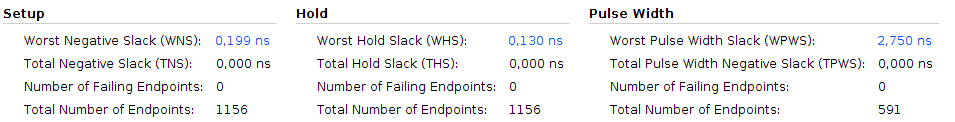
\includegraphics[width=0.7\textwidth]{figures/timing_report.png}
	\caption{Timing report}
	\label{fig:tr}
\end{figure*}

\subsection{Confronto con HLS}
Tra le due tipologie di sintesi si riscontra una sostanziale differenza nell’utilizzo delle risorse \ref{fig:ruhls}\ref{fig:ru}. La funzione in C++ utilizza 321 LUT in totale su 53200, mentre il sistema implementato in VHDL/verilog utilizza 725 LUT su 53200. Anche il numero di FF è calato considerevolmente, passando da 590 a 143. Quindi a livello generale la sintesi HLS risulta migliore nell’utilizzo delle risorse.

La latenza minima e la latenza massima in HLS hanno lo stesso valore, pari a 3, mentre, come detto in precedenza, in VHDL/verilog la latenza dipende da diversi fattori e non può essere determinata in modo certo.

\section{Conclusioni}
In linea generale si può dire che la sintesi della semplice funzione in C++ è risultata migliore di quella in VHDL/verilog.

L'implementazione del sistema attraverso l'utilizzo di diversi linguaggi di descrizione dell'hardware ha permesso di evidenziare le differenze e le similitudini tra di essi (ad esempio nella sintassi di verilog e di SystemC). 

\appendix

\begin{figure*}[bt]
	\centering
	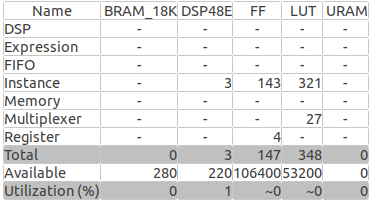
\includegraphics[width=0.7\columnwidth]{figures/resource_utilization_hls.png}
	\caption{Resource utilization HLS}
	\label{fig:ruhls}
\end{figure*}

\begin{figure*}[bt]
	\centering
	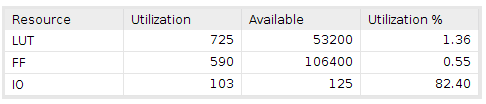
\includegraphics[width=0.7\textwidth]{figures/resource_utilization.png}
	\caption{Resource utilization}
	\label{fig:ru}
\end{figure*}

\begin{figure*}[bt]
	\centering
	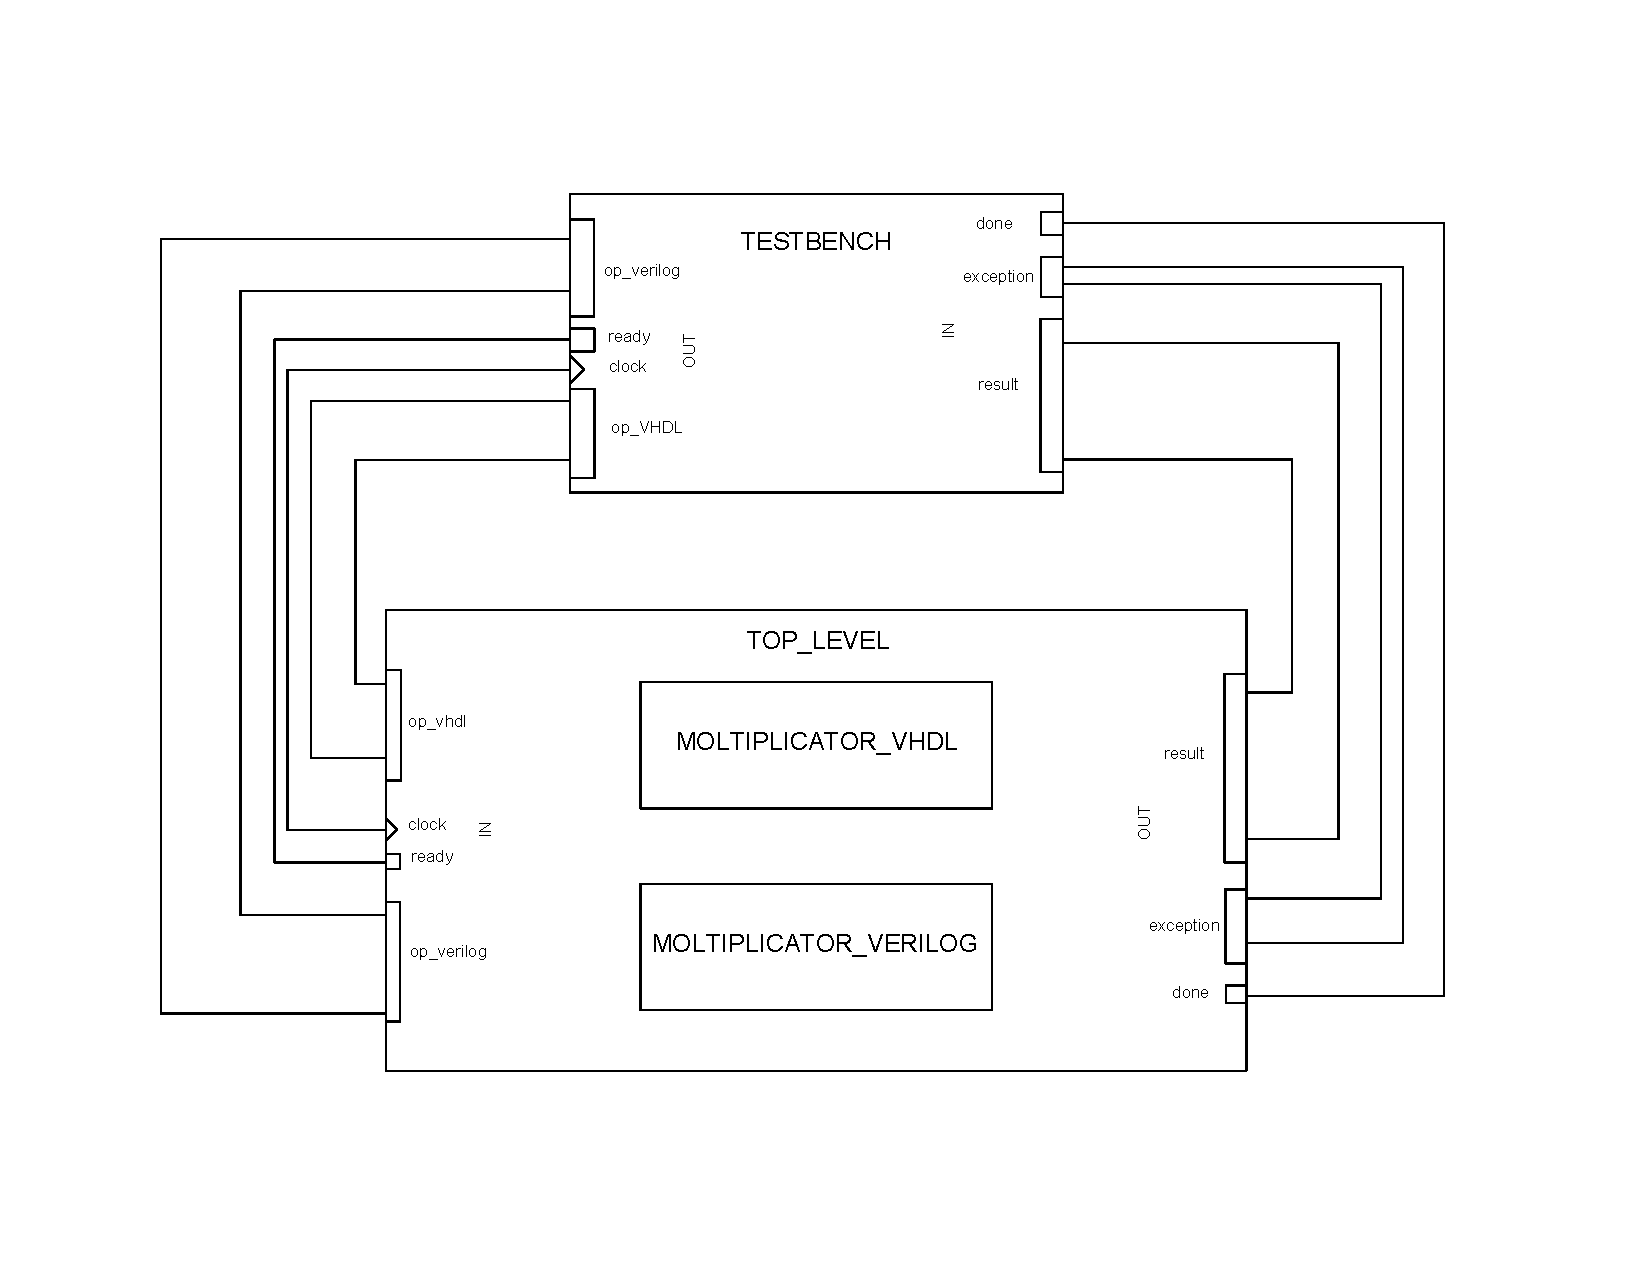
\includegraphics[width=\textwidth]{figures/abstract.pdf}
	\caption{Sistema a livello astratto}
	\label{fig:abstract}
\end{figure*}

\begin{figure*}[bt]
	\centering
	\includegraphics[width=\textwidth]{figures/efsm_mul.png}
	\caption{EFSM moltiplicatore}
	\label{fig:efsmmul}
\end{figure*}

\begin{figure*}[bt]
	\centering
	\includegraphics[width=\columnwidth]{figures/efsm_tl.png}
	\caption{EFSM top level}
	\label{fig:efsmtl}
\end{figure*}

\begin{figure*}[bt]
	\centering
	
\includegraphics[width=\textwidth]{figures/fsmd_tl.png}
	\caption{FSMD top level}
	\label{fig:fsmdtl}
\end{figure*}

\begin{figure*}[bt]
	\centering
	
\includegraphics[width=\textwidth]{figures/fsmd_mul.png}
	\caption{FSMD moltiplicatore}
	\label{fig:fsmdmul}
\end{figure*}

\end{document}